%!Mode:: "TeX:UTF-8"
\section{内存管理}
\subsection{虚拟内存}
虚拟内存是一种将内存组织(memory organization)同物理硬件解耦的方法。
产生的作用包括:访问保护,内存共享,屏蔽物理组织(屏蔽主存与二级存储直接的交换,注意两级存储都叫memory,虚拟内存实际上是virtual memory)。

\subsection{内存池}
malloc和operator new等动态内存分配接口存在外部碎片等问题,考虑到性能原因,不适合用于实时系统。
更有效的方式是使用内存池分配。
有许多实时操作系统采用了内存池,IBM 的 Transaction Processing Facility 便是其中一个例子。
Nginx等系统中,内存池这一术语指的是region,即一组变长分配被一次释放。

内存池的分配函数,可以不仅仅返回地址,而是返回一个handle。比如handle实现为一个无符号整型,可切割为池号、块号和版本号。版本号用于检测内存块的重复释放。
多个内存池可以防止树状结构中。

内存池的缺点是产生内部碎片,尤其对大块而言浪费显著。此外,内存池还必须针对具体应用进行tune。
相对malloc,内存池的优点是:诸多同类型对象所需的内存,只需调用一次malloc和一次free(chunking技术);针对同一类型的频繁分配释放,有常数操作时间;不需占用额外空间的管理信息(对于小块而言管理信息意味着利用率低效)。

\subsection{伙伴系统}
伙伴块分配技术:
In this system, memory is allocated into several pools of memory instead of just one, where each pool represents blocks of memory of a certain power of two in size. All blocks of a particular size are kept in a sorted linked list or tree and all new blocks that are formed during allocation are added to their respective memory pools for later use. If a smaller size is requested than is available, the smallest available size is selected and halved. One of the resulting halves is selected, and the process repeats until the request is complete. When a block is allocated, the allocator will start with the smallest sufficiently large block to avoid needlessly breaking blocks. When a block is freed, it is compared to its buddy. If they are both free, they are combined and placed in the next-largest size buddy-block list.
一个内存块被释放时,需要找到其buddy,判断是否合并。通过一个异或运算即可找到其buddy。

Linux用伙伴系统来管理连续页帧。为了在同一页帧内部的小对象分配,早期的Linux使用13个几何分布内存池(块长均为2的幂,32字节到128KB),而伙伴系统用于向内存池供给。
后来Linux改用slab分配器。

\subsection{slab分配器}
slab分配器最早被Solaris2.4被 Jeff Bonwick 引入,广泛用于Unix类操作系统,包括Linux。Linux自2.6.23版本开始以SLUB分配器代替slab分配器作为默认分配器。
Jeff 发现对内核中普通对象进行初始化所需的时间超过了对其进行分配和释放所需的时间。因此他的结论是不应该将内存释放回一个全局的内存池,而是将内存保持为针对特定目而初始化的状态。例如,如果内存被分配给了一个互斥锁,那么只需在为互斥锁首次分配内存时执行一次互斥锁初始化函数(mutex\_init)即可。

每一种类型的对象对应的存储系统成为一个cache(\verb$kmem_cache_t$类型)。每一个对象的cache系统由一个或多个slab构成,每个slab是一组连续的页帧,容纳多个对象块。
内核中用slab分配器提供内存的资源包括进程描述字,文件描述符,信号量等。内核周期性扫描各cache,释放空的slab。

\begin{figure}[ht]
	\begin{center}
		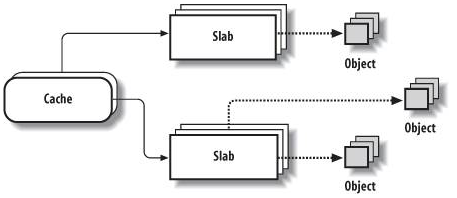
\includegraphics[keepaspectratio,width=0.3\paperwidth]{Pictures/Kernel/LinuxSlabAllocator.png}
		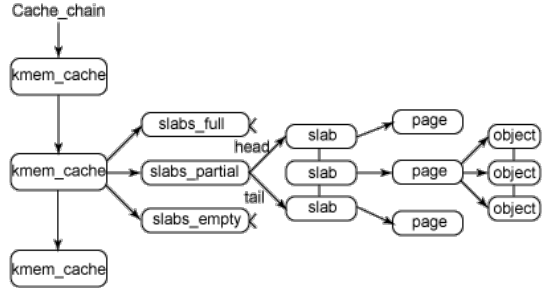
\includegraphics[keepaspectratio,width=0.3\paperwidth]{Pictures/Kernel/LinuxKmemSlab.png}
		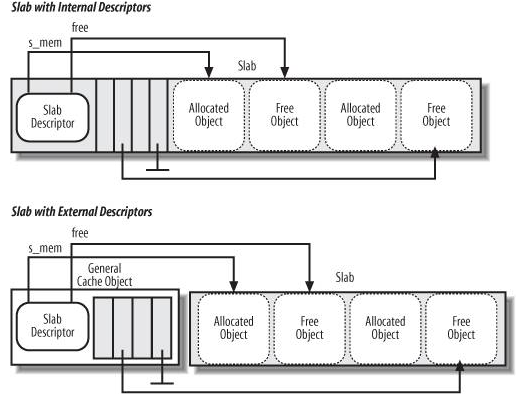
\includegraphics[keepaspectratio,width=0.3\paperwidth]{Pictures/Kernel/SlabAndObjects.png}
	    \caption{Linux内核slab分配器结构}
	\label{fig:LinuxSlabAllocator}
	\end{center}
\end{figure}



Memcached用slab分配器作内存管理。注意网上谈论的slab分配器多是memcached的分配器,而不是Linux内核的。
\begin{figure}[ht]
	\begin{center}
		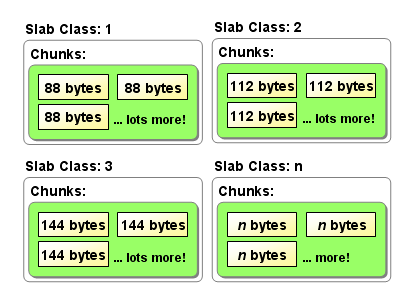
\includegraphics[keepaspectratio,width=0.3\paperwidth]{Pictures/Kernel/slabAndChunk.png}
	\caption{Memcached:slab和chunk}
	\label{fig:slabAndChunk}
	\end{center}
\end{figure}




与传统的内存管理模式相比,slab缓存分配器提供了很多优点。首先,内核通常依赖于对小对象的分配,它们会在系统生命周期内进行无数次分配。slab缓存分配器通过对类似大小的对象进行缓存而提供这种功能,从而避免了常见的碎片问题。slab分配器还支持通用对象的初始化,从而避免了为同一目而对一个对象重复进行初始化。最后,slab分配器还可以支持硬件缓存对齐和着色,这允许不同缓存中的对象占用相同的缓存行,从而提高缓存的利用率并获得更好的性能。


Linux内核中,slab分配器具体用法可以这样:
\begin{lstlisting}[language=C++]
struct kmem_cache *cachep = NULL;
cachep = kmem_cache_create("cache_name", 
  sizeof(struct mystruct), 0, SLAB_HWCACHE_ALIGN, NULL, NULL);
struct yourstruct *bodyp = NULL;
bodyp = (struct yourstruct *) kmem_cache_alloc(cachep, 
  GFP_ATOMIC & ~__GFP_DMA);
// .... use bodyp
kmem_cache_free(cachep, bodyp);
// .... other stuff
kmem_cache_destroy(cachep);
\end{lstlisting}


proc文件系统提供了一种简单的方法来监视系统中所有活动的 slab 缓存。这个文件称为 /proc/slabinfo,
它除了提供一些可以从用户空间访问的可调整参数之外,还提供了有关所有slab缓存的详细信息。
要调优特定的slab缓存,可以简单地向 /proc/slabinfo 文件中以字符串的形式回转slab缓存名称和3个可调整的参数。
格式为 “cacheName limit batchcount sharedfactor”:
\begin{verbatim}
# echo "my_cache 128 64 8" > /proc/slabinfo
\end{verbatim}
limit字段表示每个CPU可以缓存的对象的最大数量。
batchcount字段是当缓存为空时转换到每个CPU缓存中全局缓存对象的最大数量。sharedfactor参数说明了SMP系统的共享行为。





Linux内核之内存管理
\url{http://www.360doc.com/content/13/0414/15/7044580_278199905.shtml}

\subsection{slab, slub和slob}

Slab是基础,是最早从Sun OS那引进的;Slub是在Slab上进行的改进,在大型机上表现出色;而Slob(Simple List Of Blocks)是针对小型系统设计的,主要是嵌入式。


SLAB是Linux上一个古老的内存分配器。因为其结构复杂,所以几乎没有人敢修改它。
众所周知,操作系统进行内存分配的时候,是以页为单位进行的,也可以称为内存块或者堆。但是内核对象远小于页的大 小,而这些对象在操作系统的生命周期中会被频繁的申请和释放,并且实验发现,这些对象初始化的时间超过了分配内存和释放内存的总时间,所以需要一种更细粒 度的针对内核对象的分配算法,于是SLAB诞生了:
SLAB缓存已经释放的内核对象,以便下次申请时不需要再次初始化和分配空间,类似对象池的概念。并且没有修改通用的内存分配算法,以保证不影响大内存块分配时的性能。

SLAB最上层为一个由多个kmem\_cache组成的cache chain。
每个kmem\_cache由slabs\_full,slabs\_partial,slabs\_empty这3个队列组成,分别标记slab全部已被分配的 页,部分被分配的页,为分配slab的页。显然,一个新的slab申请到达时,slab\_partial页会被考虑;一个内存块释放时, slab\_empty将被优先考虑。

由于SLAB按照对象的大小进行了分组,在分配的时候不会产生堆分配方式的碎片,也不会产生Buddy分配算法中的空间浪费,并且支持硬件缓存对齐来提高TLB的性能,堪称完美。
但是这个世界上没有完美的算法,一个算法要么占用更多的空间以减少运算时间,要么使用更多的运算时间减少空间的占用。优秀的算法就是根据实际应用情况在这 两者之间找一个平衡点。SLAB虽然能更快的分配内核对象,但是metadata,诸如缓存队列等复杂层次结构占用了大量的内存。

SLUB("the unqueued slab allocator") 因此而诞生:
SLUB 不包含SLAB这么复杂的结构。SLAB不但有队列,而且每个SLAB开头保存了该SLAB对象的metadata。SLUB只将相近大小的对象对齐填入页面,并且保存了未分配的SLAB对象的链表,访问的时候容易快速定位,省去了队列遍历和头部metadata的偏移计算。该链表虽然和SLAB一样是每 CPU节点单独维护,但使用了一个独立的线程来维护全局的SLAB对象,一个CPU不使用的对象会被放到全局的partial队列,供其他CPU使用,平 衡了个节点的SLAB对象。回收页面时,SLUB的SLAB对象是全局失效的,不会引起对象共享问题。另外,SLUB采用了合并相似SLAB对象的方法, 进一步减少内存的占用。

据内核开发人员称,SLUB相对于SLAB有5\%-10\%的性能提升和减少50\%的内存占用。所以SLUB是一个时间和空间上均有改善的算法,而且SLUB完全兼容SLAB的接口,所以内核其他模块不需要修改即可从SLUB的高性能中受益。SLUB在2.6.22内核中理所当然的替代了SLAB。

SLAB 分配器多年以来一直位于 Linux 内核的内存管理部分的核心地带,内核黑客们一般不愿意主动去更改它的代码,因为它实在是非常复杂,而且在大多数情况下,它的工作完成的相当不错。但是,随着大规模多处理器系统和 NUMA系统的广泛应用,SLAB 分配器逐渐暴露出自身的严重不足:
1. 较多复杂的队列管理。在 SLAB 分配器中存在众多的队列,例如针对处理器的本地对象缓存队列,slab 中空闲对象队列,每个 slab 处于一个特定状态的队列中,甚至缓冲区控制结构也处于一个队列之中。有效地管理这些不同的队列是一件费力且复杂的工作。

2. slab 管理数据和队列的存储开销比较大。每个 slab 需要一个 struct slab 数据结构和一个管理所有空闲对象的 kmem\_bufctl\_t(4 字节的无符号整数)的数组。当对象体积较少时,kmem\_bufctl\_t 数组将造成较大的开销(比如对象大小为32字节时,将浪费 1/8 的空间)。为了使得对象在硬件高速缓存中对齐和使用着色策略,还必须浪费额外的内存。同时,缓冲区针对节点和处理器的队列也会浪费不少内存。测试表明在一个 1000 节点/处理器的大规模 NUMA 系统中,数 GB 内存被用来维护队列和对象的引用。

3. 缓冲区内存回收比较复杂。

4. 对 NUMA 的支持非常复杂。SLAB 对 NUMA 的支持基于物理页框分配器,无法细粒度地使用对象,因此不能保证处理器级缓存的对象来自同一节点。

5. 冗余的 Partial 队列。SLAB 分配器针对每个节点都有一个 Partial 队列,随着时间流逝,将有大量的 Partial slab 产生,不利于内存的合理使用。

6. 性能调优比较困难。针对每个 slab 可以调整的参数比较复杂,而且分配处理器本地缓存时,不得不使用自旋锁。

7. 调试功能比较难于使用。

为了解决以上 SLAB 分配器的不足之处,内核开发人员 Christoph Lameter 在 Linux 内核 2.6.22 版本中引入一种新的解决方案:SLUB 分配器。
SLUB 分配器特点是简化设计理念,同时保留 SLAB 分配器的基本思想:每个缓冲区由多个小的 slab 组成,每个 slab 包含固定数目的对象。SLUB 分配器简化了kmem\_cache,slab 等相关的管理数据结构,摒弃了SLAB 分配器中众多的队列概念,并针对多处理器、NUMA 系统进行优化,从而提高了性能和可扩展性并降低了内存的浪费。为了保证内核其它模块能够无缝迁移到 SLUB 分配器,SLUB 还保留了原有 SLAB 分配器所有的接口 API 函数。


\subsection{Bélády's anomaly}
所谓\textbf{Belady}现象是指:采用FIFO算法(选择装入最早的页面置换)时,如果对—个进程未分配它所要求的全部页面,有时就会出现分配的页面数增多但缺页率反而提高的异常现象。
原因是,增加了页帧后,本应丢失的帧被命中,但逐渐移到队头,而不是追加到队尾,改变了各帧的相对顺序,后果比较复杂。












\clearpage

